%!TEX root = ../../../adrien_gomar_phd.tex
\chapter{Advantages of Fourier-based time methods}
\label{cha:advantages}

\chabstract{In this chapter, the advantage of using the 
harmonic balance approach to estimate the 
temporal derivative is assessed. First, an analytical
function, whose derivative is known, is chosen to
compare the accuracy of the estimation of the derivative
using the harmonic balance operator
and two finite-difference schemes. It is shown that 
the HB operator is spectral accurate. The same
function is then used along with the linear advection toy problem
to ensure that this property is kept when iteratively solving
an equation. Finally, a function composed of two segregated frequencies
is tested. It is shown that the multi-frequential approach
is well suited to this sort of problems and gives a CPU
gain, compared to a mono-frequential HB method, that is proportional
to the segregation of the frequencies. This properties
justifies the used of such an approach in the framework of the
current thesis.}

\minitoc
\newpage


\section{Comparison of the harmonic balance operator and finite difference schemes}
\label{sec:hb_operator}
%!TEX root = ../../../adrien_gomar_phd.tex

To assess the capability of the HB operator, used in the present work, to
provide accurate approximations of the time-derivative, 
we consider the simple example of a pure
five-harmonic signal of the form:
\begin{equation}
    \label{eq:sum_sin}
    u(t) = \cos(\omega t) + \sin(2 \omega t) +
    \cos(3 \omega t) + \sin(4 \omega t) + \cos(5 \omega t),
\end{equation}
where $\omega = 2 \pi f$ and $f$ is the temporal frequency of
the considered phenomenon.
The analytical derivative is then:
\begin{equation}
    \label{eq:sum_sin_deriv}
    \frac{\partial u}{\partial t} = 
    \omega\left[ -\sin(\omega t) + 
    2\cos(2 \omega t) -
    3\sin(3 \omega t) + 
    4\cos(4 \omega t) -
    5\sin(5 \omega t)\right].
\end{equation}
The exact derivative is compared to the approximated derivative by applying 
the HB operator defined in Eq.~\eqref{eq:sm_hb_mono_source_term_matrix}
and two different Finite-Difference (FD) schemes,
a second-order centered scheme:
\begin{equation}
    \frac{\partial u}{\partial t} (t=t_q) \approx 
    \frac{u_{q+1} - u_{q-1}}{2 \Delta t},
    \label{eq:hb_op_center2}
\end{equation}
and a fourth-order centered scheme:
\begin{equation}
    \frac{\partial u}{\partial t} (t=t_q) \approx 
    \frac{-u_{q+2} + 8 u_{q+1} - 8 u_{q-1} + u_{q-2}}{12\Delta t}.
    \label{eq:hb_op_center4}
\end{equation}

For finite-difference schemes, 
we assume that the time line is discretized 
by a regular mesh of step $\Delta t$, such that $t_q = q \Delta t$.
Figure~\ref{fig:hb_operator_sample} shows the resulting approximations 
of the derivative over one period.
\begin{figure}[htb]
  \centering
  \subfigure[HB]{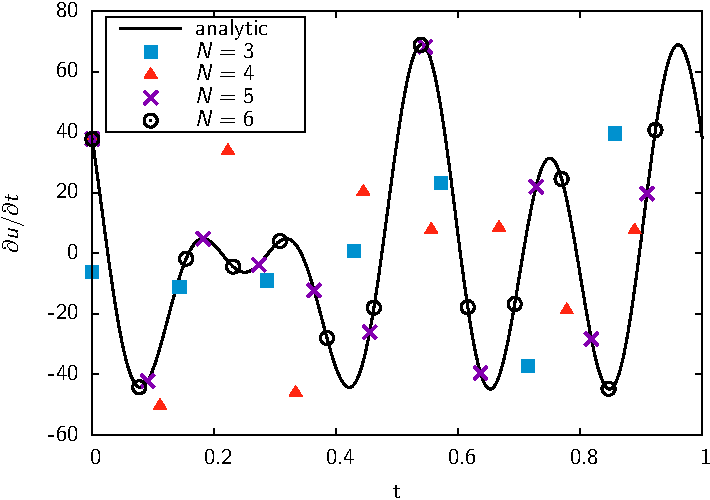
\includegraphics[width=.3\textwidth]{HB_OPERATOR_PPT_HB.pdf}}
  \subfigure[FD 2\textsuperscript{nd} order]{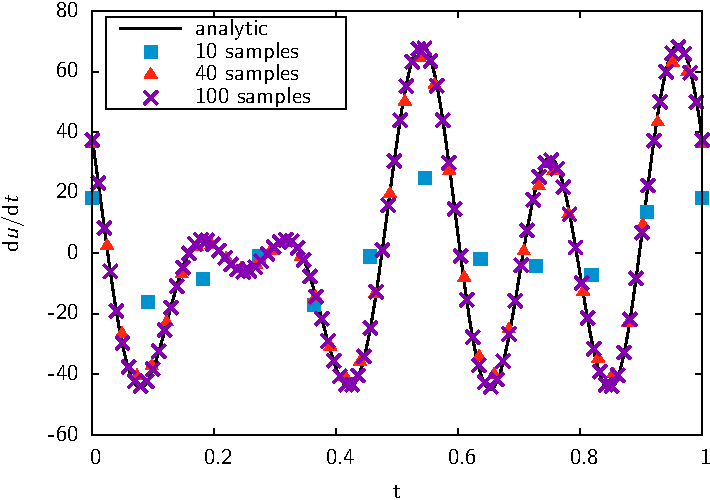
\includegraphics[width=.3\textwidth]{HB_OPERATOR_PPT_FD2.pdf}}
  \subfigure[FD 4\textsuperscript{th} order]{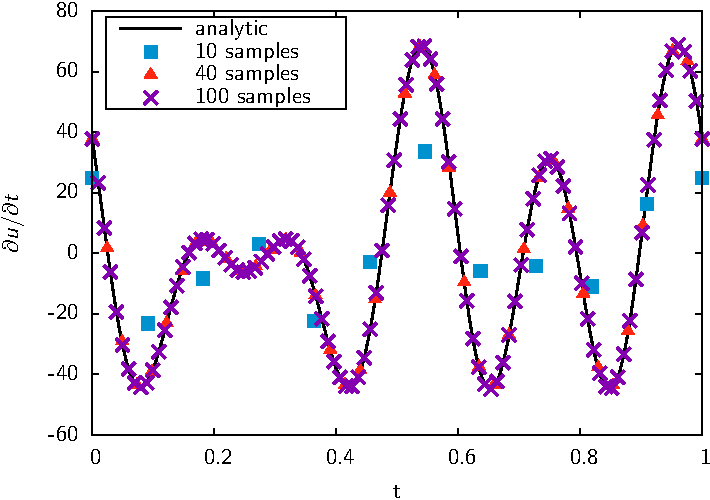
\includegraphics[width=.3\textwidth]{HB_OPERATOR_PPT_FD4.pdf}}
  \caption{Time-derivative estimation by the harmonic balance operator,
  the 2\textsuperscript{nd} order and 4\textsuperscript{th} finite-difference schemes.}
  \label{fig:hb_operator_sample}
\end{figure}
Four sampling levels
are tested for the HB operator: 7, 9, 11 and 13~time instances per period
corresponding to, respectively, $N=3$, 4, 5 and 6.
For the FD schemes, the periodicity time interval is sampled by
10, 40 and 100 points.
For 40~samples, the 4\textsuperscript{th} order FD
scheme almost fits the analytical solution. On the other-hand,
the HB operator prediction is superimposed with the analytical solution
by using 11~samples, i.e. $N=5$. Beyond that, further increasing the
number of harmonics (or samples)
does not improve the solution.

To quantitatively analyze the results, the 
$\mathcal{L}_2$-norm of the absolute error with respect to the analytical
derivative is computed for the different schemes and 
sampling levels (see Fig.~\ref{fig:hb_operator_error}).
\begin{figure}[htb]
  \centering
   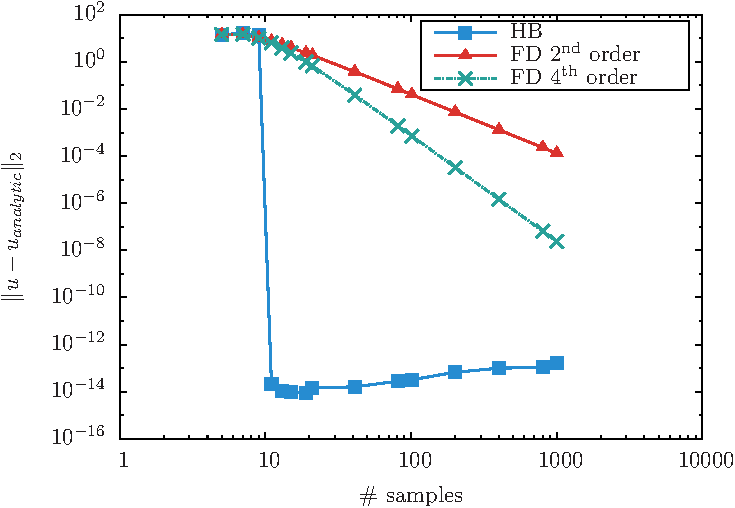
\includegraphics[width=.4\textwidth]{HB_OPERATOR_ERROR.pdf}
   \caption{$\mathcal{L}_2$-norm of the error for each time-derivative
   schemes.}
  \label{fig:hb_operator_error}
\end{figure}
As expected, the error of the 4\textsuperscript{th}~order FD
decreases faster  than the 2\textsuperscript{nd}~order for a given sampling level.
When the number of harmonics is low 
(i.e. $N < 5$), the error is high. But as soon as $N \geq 5$, the error
drastically decreases to machine precision.
This illustrates the spectral accuracy as explained in 
Sec.~\ref{sec:spectral_accuracy}. In fact, the function defined
in Eq.~\eqref{eq:sum_sin_deriv} approximated by the spectral operator
is infinitely differentiable and periodic in $[0, T]$.
Thus, using the properties established in Sec.~\ref{sec:spectral_accuracy},
the convergence rate of the spectral operator is $\mathcal{O} (k^{-\infty})$
for $k > k_0$, here $k_0=5$. In this case, $k_0$
reflects the frequency content of the signal (namely $5$ harmonics).


\section{Periodic advection of a sum of sine functions}
\label{sec:sum_sine}
%!TEX root = ../../../adrien_gomar_phd.tex



\section{Capturing a segregated multi-frequential signal}
\label{sec:adv_multifreq}
%!TEX root = ../../../adrien_gomar_phd.tex

\mytodo{Reponse forcee => multiple de freq de revolution, + mettre ratio frequence
calcul dream AEL}

In Section~\ref{sec:sm_hb_multi}, the multi-frequential harmonic
balance approach has been presented. In this method,
the frequencies can be chosen arbitrarily. This becomes particularly
interesting when dealing with signal/ flow field composed of segregated
frequencies. For instance, let us consider the linear advection toy problem
as defined in Sec.~\ref{sec:toy_convection} with 
a perturbation 
in the form of a sum of two sine functions,
applied at the left boundary:
\begin{equation}
    u_l(t) = \sin(\omega t) + \sin(22 \omega t).
    \label{eq:multifreq_inj_func}
\end{equation}

\subsection{Toward aeroelasticity of contra-rotating open rotors}
The reason why we studied the multi-frequential harmonic balance
approach for the aeroelasticity of contra-rotating open rotors
is that it is a problem where the major frequencies are most
likely to be segregated as shown previously in Chap.~\ref{cha:cror} and
Chap.~\ref{cha:ael}. In this framework, the multi-frequential
harmonic balance approach looks very promising according to the results
seen in this Chapter.

\subsection{Using a mono-frequential approach}

Obviously, computing the advection of such a signal using
a classical time-marching scheme would require to discretize the
smaller period. The largest frequency
(here $f_2 = 22$~Hz) acts as a bottleneck as the time-step will be chosen
according to this frequency. The cost scales thus with the ratio of $f_2 / f_1 = 22$. This
means that compared to a computation where only $f_1$ or only $f_2$
is involved, the cost will be multiplied by~ \mbox{$(2 \times 22 + 1) / (2 \time 1+1) = 9$}.

This holds true when computing the solution with the mono-frequential
harmonic balance approach. In fact, the frequencies can not be chosen arbitrarily.
Therefore, to compute such a configuration, a $N=22$ harmonic computation
will be needed to be spectral accurate. To emphasize that, mono-frequential
HB computations are run with 1 to 25~harmonics.
As made in the Section~\ref{sec:sum_sine}, 
for six chosen computations of the~25 computations, 
we show spatial distributions of the solution
at three time instances, namely, $t=0$, $t=T/3$ and $t=2T/3$.
It is shown in Fig.~\ref{fig:inj_multifreq_tsm}.
\begin{figure}[htb]
  \centering
  \subfigure[$N=1$]{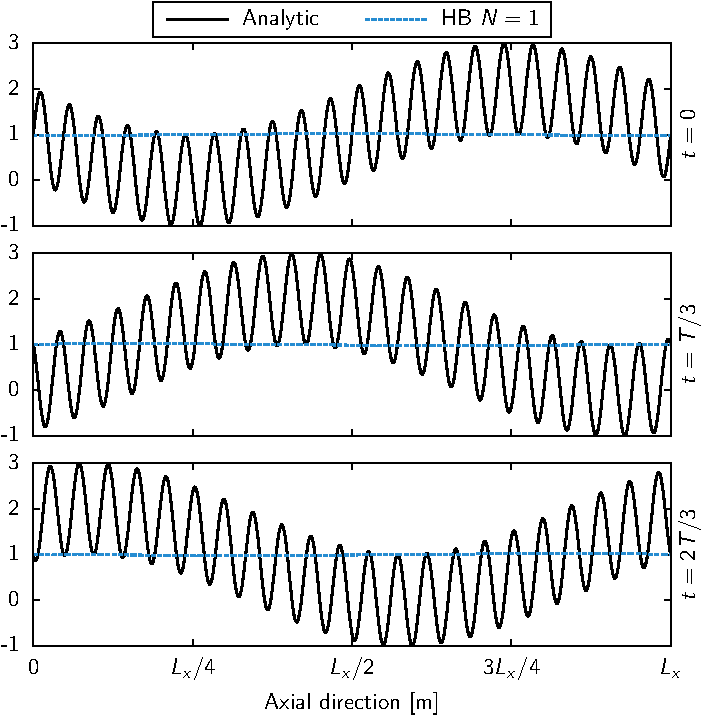
\includegraphics[width=.35\textwidth]{convection_multifreq_tsm_N1.pdf}}
  \subfigure[$N=5$]{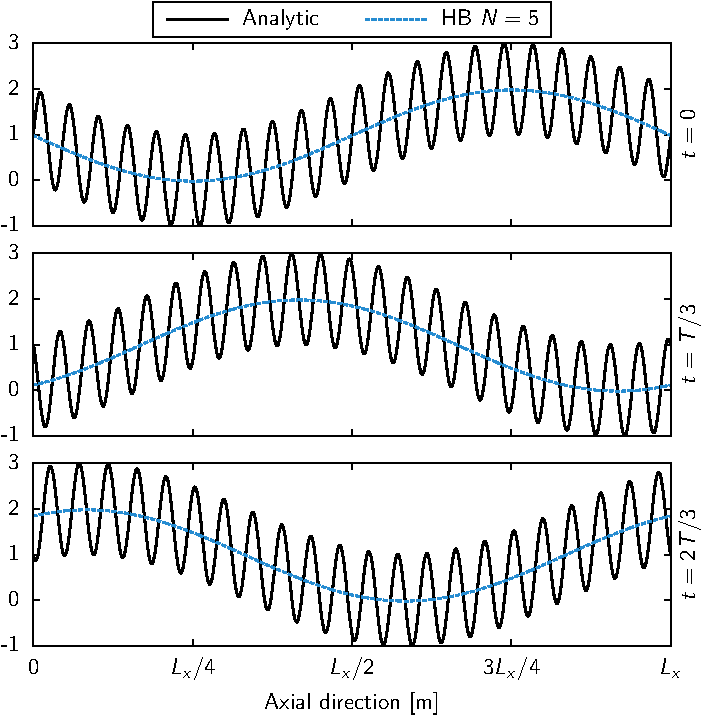
\includegraphics[width=.35\textwidth]{convection_multifreq_tsm_N5.pdf}}
  \subfigure[$N=11$]{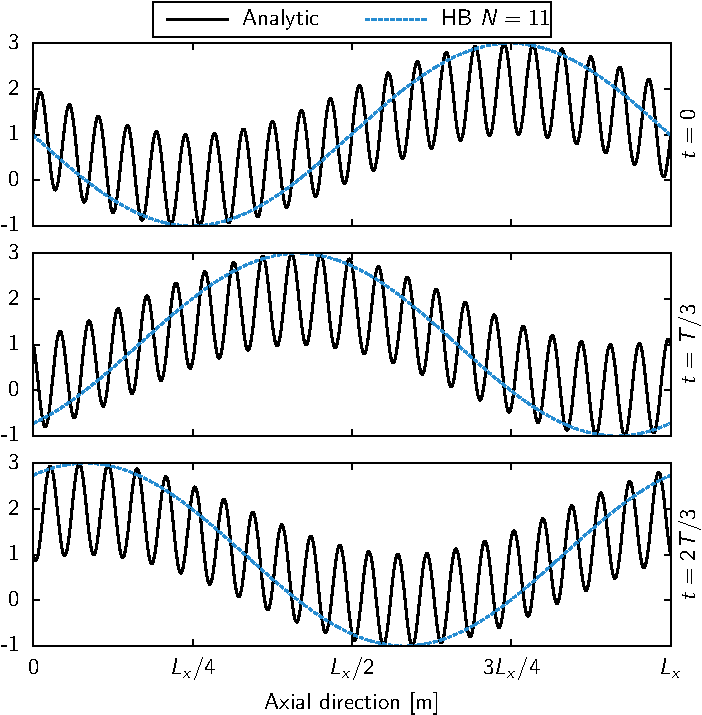
\includegraphics[width=.35\textwidth]{convection_multifreq_tsm_N11.pdf}}
  \subfigure[$N=16$]{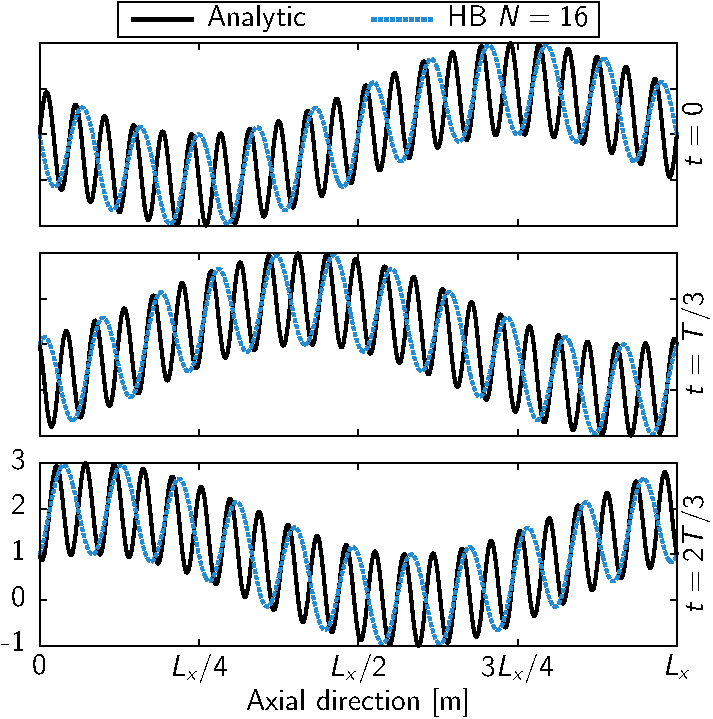
\includegraphics[width=.35\textwidth]{convection_multifreq_tsm_N16.pdf}}
  \subfigure[$N=22$]{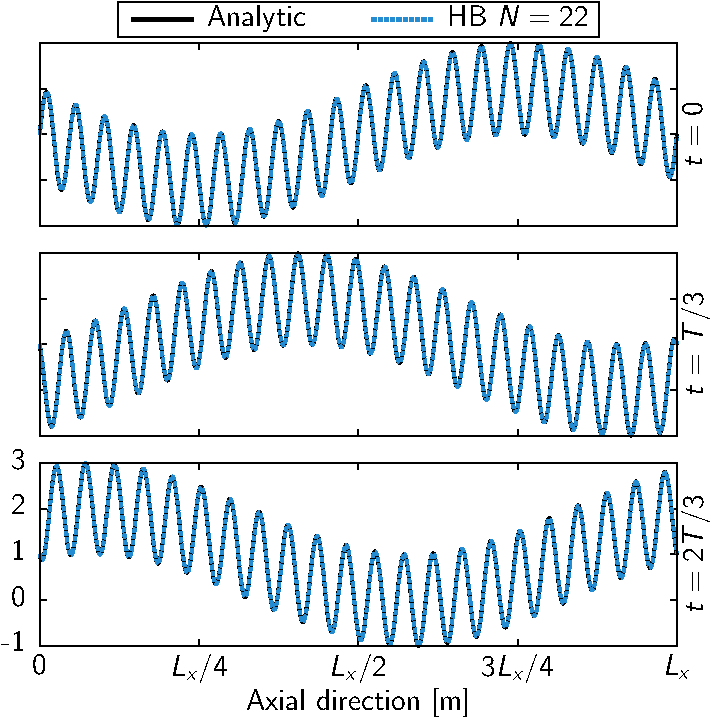
\includegraphics[width=.35\textwidth]{convection_multifreq_tsm_N22.pdf}}
  \subfigure[$N=23$]{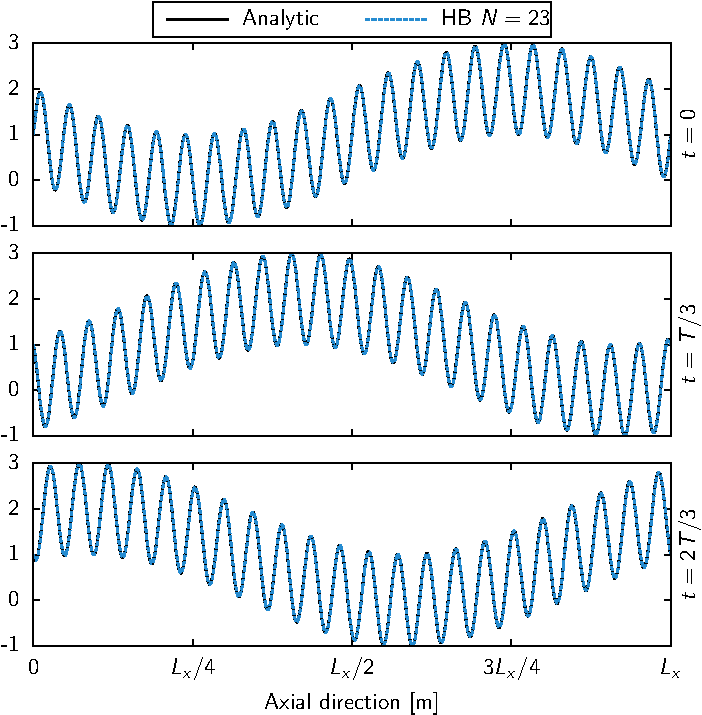
\includegraphics[width=.35\textwidth]{convection_multifreq_tsm_N23.pdf}}
  \caption{Linear advection of a sum of two segregated sine functions: 
  numerical solutions at different time instances for different numbers of harmonics.}
  \label{fig:inj_multifreq_tsm}
\end{figure}
Again, the accuracy in capturing the injected function
improves with the number of harmonics,
until it reaches the frequency content
of the injected signal, i.e. 22~harmonics.
After that, the results of the HB computations are
superimposed with the analytical solution. 
The problem, with such a segregation of frequencies, is that 
the mono-frequential version suffers the same
problems as a classical time-marching scheme in terms of 
computational cost.

To quantitatively analyze the results,
the discrete $\mathcal{L}_2$-norm of the error 
in time is computed over all the time instances
at each grid points over the domain.
Then, the average in space is computed.
It is shown in Fig.~\ref{fig:conv_multifreq_tsm} for the
mono-frequential HB computations ranging from one to~25
harmonics.
\begin{figure}[htb]
  \centering
  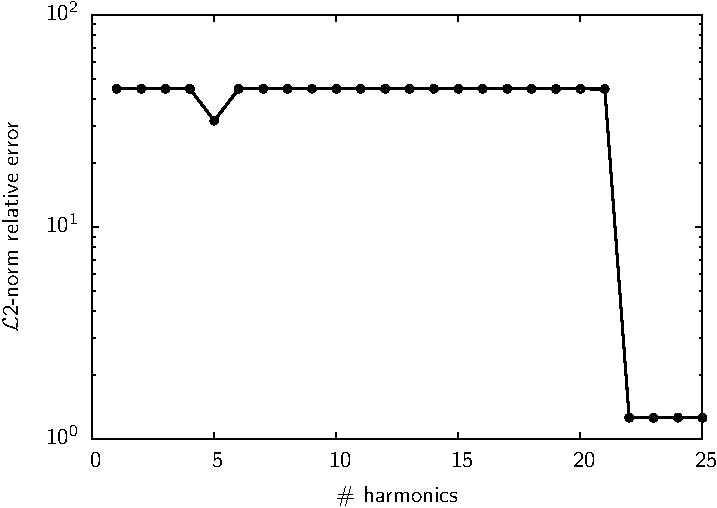
\includegraphics[width=.5\textwidth]{convection_multifreq_error.pdf}
  \caption{Linear advection of a sum of two segregated sine functions: convergence of the mono-frequential HB method error.}
  \label{fig:conv_multifreq_tsm}
\end{figure}
When the number of harmonics
used to compute the solution is higher than the content of the spectrum,
then the error decreases drastically. The spectral accuracy is retrieved
but only starting at $N=22$.
In fact, similar as in Sec.~\ref{sec:sum_sine},
the injected function is indefinitely differential and periodic
leading an infinite convergence slope. We can observe a slight local convergence
for the $N=5$ harmonics HB computation. This is due to the fortunate 
capture of the low-frequency pattern of the injected function.

\subsection{Using a multi-frequential approach}

One of the advantage of the multi-frequential HB method introduced in Sec.~\ref{sec:sm_hb_multi}
and used in this thesis is that it can take arbitrary frequencies into account.
In the case of an injected signal with a large frequency segregation, the
benefit might be tremendous. Let us consider again the signal defined in 
Eq.~\eqref{eq:multifreq_inj_func} and compute one HB simulation using 
$f_1=1$~Hz and $f_2=22$~Hz as input frequencies. This gives a computation
of two coupled calculation
that is nine times faster than the $N=22$ converged mono-frequential
HB computation.
Again
we show spatial distributions of the solution
at three time instances, namely, $t=0$, $t=T/3$ and $t=2T/3$
in Fig.~\ref{fig:inj_multifreq_hb}.
\begin{figure}[htb]
  \centering
  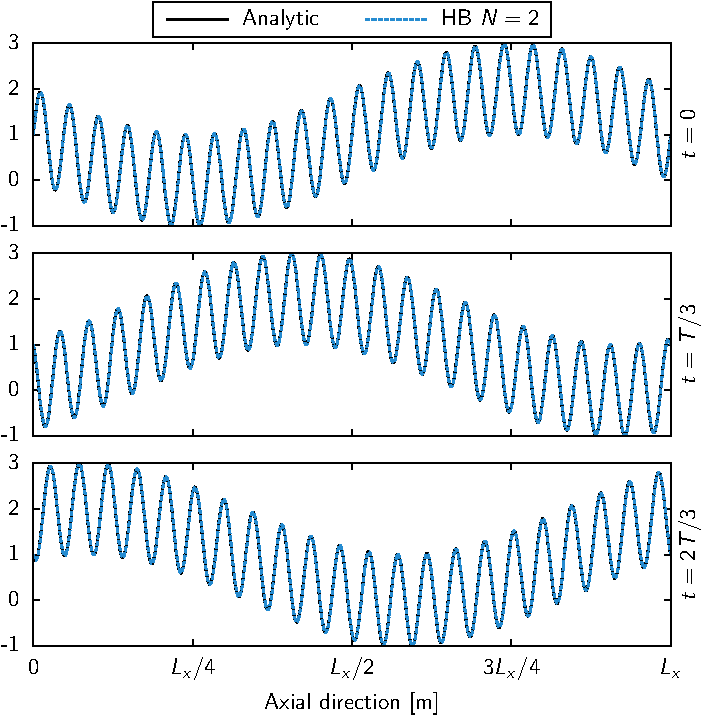
\includegraphics[width=.5\textwidth]{convection_multifreq_hbt_N2.pdf}
  \caption{Linear advection of a sum of two segregated sine functions: 
  numerical solutions at different time instances for different numbers of harmonics using the
  multi-frequential harmonic balance method.}
  \label{fig:inj_multifreq_hb}
\end{figure}
With only two input frequencies, the multi-frequential
HB solution is superimposed with the analytical solution.
Moreover, the $\mathcal{L}2$-norm of the error is 
exactly the same as the one of the $N=22$ mono-frequential
approach.
\mytodo{conclusion partielle: c'est trop cool !! -> rapprocher de Campbell}


\chconclu{The advantages of Fourier-based time methods
is shown in this chapter. When dealing with periodic functions
that have some regularity properties, Fourier-based time methods
(namely here the harmonic balance) are spectral accurate: they are
able to capture a signal with the smallest error by using a finite
number of harmonics. When dealing with a multi-frequential signal whose
frequencies is largely segregated, the use of the multi-frequential
version of the harmonic balance gives a tremendous gain in CPU time as
only the frequencies involved in the computation have to be set.
In opposite, the mono-frequential (and also the classical time-marching schemes)
need to discretize all the intermediate frequencies. Hence the choice of the multi-frequential
harmonic balance approach for this work.}
